%% ==========================================================
%% SAT-Based Sudoku Solving: A Comparative Analysis of
%% At-Most-One Encodings and Exact Optimisation Methods
%%
%% Elsevier elsarticle – Overleaf ready.
%% Upload this file + all PNG figures to the same Overleaf folder.
%% Compiler: pdfLaTeX
%% ==========================================================
\documentclass[preprint,10pt,authoryear]{elsarticle}
%% Body text = 10pt.  Section headings are explicitly set below.

%% ---- Core packages ------------------------------------------
\usepackage{amsmath,amssymb,amsthm}
\usepackage{booktabs}
\usepackage{multirow}
\usepackage{graphicx}
\usepackage{xcolor}
\usepackage{hyperref}
\usepackage{microtype}
\usepackage{array}
\usepackage[utf8]{inputenc}
\usepackage[T1]{fontenc}
\usepackage{float}           % [H] forced placement
\usepackage{caption}

\usepackage{algorithm}
\usepackage{algpseudocode}

%% ---- Heading hierarchy (requires titlesec) -------------------
%% section   : 15pt bold,  1.5× body
%% subsection: 13pt bold,  1.3× body
%% subsubsect: 11pt bold-italic
\usepackage[explicit]{titlesec}
\titleformat{\section}
  {\fontsize{15}{18}\bfseries}{\thesection}{0.8em}{#1}
\titleformat{\subsection}
  {\fontsize{13}{15.6}\bfseries}{\thesubsection}{0.7em}{#1}
\titleformat{\subsubsection}
  {\fontsize{11}{13.2}\bfseries\itshape}{\thesubsubsection}{0.6em}{#1}
\titleformat{\paragraph}[runin]
  {\normalsize\bfseries}{}{0pt}{#1.\ }

\titlespacing{\section}{0pt}{14pt plus 4pt minus 2pt}{6pt plus 2pt}
\titlespacing{\subsection}{0pt}{10pt plus 3pt minus 2pt}{4pt plus 1pt}
\titlespacing{\subsubsection}{0pt}{8pt plus 2pt minus 1pt}{3pt plus 1pt}

%% ---- Fix abstract font size ---------------------------------
%% elsarticle uses \small inside the abstract box; restore to \normalsize.
\makeatletter
\renewenvironment{abstract}{%
  \global\setbox\absbox\vbox\bgroup
    \hsize\textwidth
    \def\baselinestretch{1}\normalsize
    \normalfont\noindent
    {\bfseries\abstractname}\par\medskip
    \noindent\ignorespaces
}{\egroup}
\makeatother

%% ---- Theorem-like environments ------------------------------
\newtheorem{theorem}{Theorem}[section]
\newtheorem{definition}{Definition}[section]
\newtheorem{proposition}[theorem]{Proposition}

%% ---- Custom macros ------------------------------------------
\newcommand{\AMO}{\textsc{Amo}}
\newcommand{\ALO}{\textsc{Alo}}
\newcommand{\EO}{\textsc{Eo}}
\newcommand{\CDCL}{\textsc{Cdcl}}
\newcommand{\CNF}{\textsc{Cnf}}

%% ---- Caption style ------------------------------------------
\captionsetup{font=footnotesize, labelfont=bf, skip=5pt}

\journal{Computers \& Operations Research}


%% ==========================================================
\begin{document}
\begin{frontmatter}

\title{SAT-Based Sudoku Solving: A Comparative Analysis of\\
       At-Most-One Encodings and Exact Optimisation Methods\\
       Across Multiple Grid Sizes}

\author[aff1]{Hoang Thi Linh Huong\corref{cor1}}
\ead{hoangthilinhhuong1@gmail.com}

\cortext[cor1]{Corresponding author}
\affiliation[aff1]{organization={University of Engineering and Technology -- Vietnam National University (UET-VNU)},
                   addressline={Student ID: 24021509},
                   city={Hanoi},
                   country={Vietnam}}

\begin{abstract}
This paper presents a comprehensive empirical study of \emph{SAT-based solving}
applied to Sudoku puzzles across three grid sizes ($9\!\times\!9$,
$16\!\times\!16$, and $25\!\times\!25$) and compares its performance against
two established exact optimisation paradigms: Constraint Programming~(CP) and
Integer Linear Programming~(ILP/MIP).
A key contribution is the systematic evaluation of five At-Most-One~(\AMO{})
propositional encodings---\emph{Pairwise}, \emph{Binary (Log)},
\emph{Commander}, \emph{Product}, and \emph{Sequential Counter}---implemented
via the \texttt{PySAT} library and tested against eight state-of-the-art CDCL
solvers (Cadical~1.9.5 / 3.0.0, Glucose~4.x / 4.2, Kissat~4.0.4,
CryptoMiniSAT, Lingeling, MiniSAT~2.2).
Experimental results on eight benchmark instances show that compact AMO
encodings reduce clause counts by up to~76\% relative to Pairwise on
$25\!\times\!25$ grids, delivering $1.7$--$2.1\times$ solve-time speedups.
On $9\!\times\!9$ instances SAT solvers achieve 8--16\,ms, matching or
outperforming CP-SAT, while ILP is $3$--$5\times$ slower.
On $16\!\times\!16$ grids, SAT with Product encoding ($\approx\!50$\,ms)
rivals CP-SAT ($\approx\!58$\,ms) and is twice as fast as Pairwise SAT.
All 300+ experiment runs are verified correct.
Source code and data are publicly available.
\end{abstract}

\begin{keyword}
SAT solving \sep Boolean satisfiability \sep At-most-one constraint \sep
Cardinality encoding \sep Sudoku \sep Integer linear programming \sep
Constraint programming \sep PySAT \sep Cadical \sep Kissat
\end{keyword}

\end{frontmatter}


%%===========================================================
\section{Introduction}
\label{sec:intro}
%%===========================================================

The Sudoku puzzle is a canonical benchmark for combinatorial reasoning: it is
an NP-complete completion problem~\citep{Yato2003} whose compact structure
makes it an ideal testbed for comparing exact solving paradigms.
Modern exact approaches include Constraint Programming~(CP), Integer Linear
Programming~(ILP/MIP), and SAT solving.

\medskip
\noindent\textbf{SAT encoding of Sudoku.}
The core challenge lies in the \emph{propositional encoding} of
\emph{Exactly-One}~(EO) constraints: each row, column, box, and cell must
contain each value exactly once.
EO decomposes as $\text{EO}(L) = \text{ALO}(L) \wedge \text{AMO}(L)$.
While ALO is a single clause, AMO admits many encodings with different
trade-offs between clause count, auxiliary variables, and propagation strength.

\medskip
\noindent\textbf{Contributions.}
\begin{enumerate}
  \item Systematic implementation and correctness verification of five \AMO{}
        encodings (Section~\ref{sec:encoding}).
  \item Empirical comparison of eight CDCL SAT solvers on $9\!\times\!9$
        through $25\!\times\!25$ benchmarks (Section~\ref{sec:results}).
  \item Head-to-head evaluation of SAT, CP, and ILP on identical instances
        (Section~\ref{sec:comparison}).
  \item Analysis of encoding-by-grid-size interaction
        (Section~\ref{sec:discussion}).
\end{enumerate}

%%===========================================================
\section{Background and Related Work}
\label{sec:background}
%%===========================================================

\subsection{SAT Solving}

Modern SAT solvers implement Conflict-Driven Clause Learning~(\CDCL{})
\citep{Moskewicz2001}, combining unit propagation, non-chronological
backtracking, and learned clause minimisation.
Solvers used: Cadical~\citep{Biere2019},
Glucose~\citep{Audemard2009} (LBD heuristic),
Kissat~\citep{Biere2020} (SAT Competition winner 2020--2022),
CryptoMiniSAT~\citep{Soos2009} (XOR reasoning), Lingeling~\citep{Biere2013}.
All accessed through PySAT~\citep{Ignatiev2018}.

\subsection{At-Most-One Encodings}

Cardinality constraint encoding has been widely studied
\citep{Sinz2005,Bailleux2003,Klieber2007,Chen2010}.
For \AMO{}: Pairwise~\citep{Cook1971} uses $O(n^2)$ clauses; Binary
(Log)~\citep{Frisch2010} uses $O(n\log n)$ clauses but lacks arc consistency;
Commander~\citep{Klieber2007} achieves arc consistency in $O(n)$ clauses;
Product~\citep{Chen2010} uses $O(n\sqrt{n})$ clauses with $O(\sqrt{n})$ aux
variables; Sequential Counter~\citep{Sinz2005} achieves arc consistency with
exactly $4(n-1)-1$ clauses.

\subsection{Sudoku Solving}

\citet{Yato2003} proved NP-completeness of Sudoku.
SAT-based approaches were pioneered by \citet{Lynce2006}.
CP-based modelling is described by \citet{Simonis2005}.
Large-scale comparisons across multiple AMO strategies remain sparse.

%%===========================================================
\section{Problem Formulation}
\label{sec:formulation}
%%===========================================================

\begin{definition}[Sudoku Completion]
Given an $n\!\times\!n$ grid ($n=k^2$, $k\in\mathbb{Z}^+$) with some cells
pre-filled from $\mathcal{D}=\{1,\ldots,n\}$, assign all empty cells so that
every row, column, and $k\!\times\!k$ box contains each value exactly once.
\end{definition}

\paragraph{Variables.}
Boolean variable $x_{r,c,v}=\top$ iff cell $(r,c)$ holds value $v$.
Total: $n^3$ variables, indexed $\mathrm{var}(r,c,v)=n^2(r{-}1)+n(c{-}1)+v$.

\paragraph{Constraints.}
Four families of EO constraints enforce the rules:
\begin{align}
  \text{Cell:}\ &\forall r,c:\ \EO\!\bigl(\{x_{r,c,v}\mid v\!\in\!\mathcal{D}\}\bigr)\\
  \text{Row:}\ &\forall r,v:\ \EO\!\bigl(\{x_{r,c,v}\mid c\!\in\![n]\}\bigr)\\
  \text{Col:}\ &\forall c,v:\ \EO\!\bigl(\{x_{r,c,v}\mid r\!\in\![n]\}\bigr)\\
  \text{Box:}\ &\forall b,v:\ \EO\!\bigl(\{x_{r,c,v}\mid(r,c)\!\in\!B_b\}\bigr)
\end{align}
Given clues add unit clauses $\{x_{r,c,v}\}$ for pre-filled cells.

%%===========================================================
\section{AMO Encoding Strategies}
\label{sec:encoding}
%%===========================================================

Let $L=(x_1,\ldots,x_n)$ be a list of literals.

\subsection{Pairwise (Naive)}
For each $i<j$: add $(\neg x_i\vee\neg x_j)$.
Complexity: $\frac{n(n-1)}{2}$ clauses, 0 aux vars. Achieves arc consistency.

\subsection{Binary (Bitwise / Log)}
Introduce $k=\lceil\log_2 n\rceil$ aux bits $b_0,\ldots,b_{k-1}$.
For each $i\in[n]$, bit $j$: add $(\neg x_i\vee b_j)$ if bit $j$ of $i$ is~1,
else $(\neg x_i\vee\neg b_j)$.
Complexity: $n\lceil\log_2 n\rceil$ clauses, $\lceil\log_2 n\rceil$ aux vars.
\emph{Does not} achieve arc consistency.

\subsection{Commander Encoding~\citep{Klieber2007}}
Partition $L$ into groups of size $\leq k$ (default $k=4$); assign
commander $c_i$ to group~$i$.
\begin{definition}[Commander \AMO{}]
For each group $G=\{x_1,\ldots,x_m\}$ with commander $c$:
(1)~$(\neg x_i\vee c)$ for all $x_i$;
(2)~$(\neg x_i\vee\neg x_j)$ for $i<j$ in $G$;
(3)~$(\neg c\vee x_1\vee\cdots\vee x_m)$.
Recurse on commander list.
\end{definition}
Complexity: $O(n)$ clauses, $O(n/k)$ aux vars.

\subsection{Product Encoding~\citep{Chen2010}}
Arrange $n$ literals in a $p\times q$ grid ($p=\lceil\sqrt{n}\rceil$)
with row indicators $R_j$ and column indicators $C_\ell$.
\begin{definition}[Product \AMO{}]
$x_i\mapsto(\lfloor i/q\rfloor,\, i\bmod q)$.
Add: $(\neg x_i\vee R_{\lfloor i/q\rfloor})$,
     $(\neg x_i\vee C_{i\bmod q})$,
     pairwise AMO on rows $\{R_j\}$, pairwise AMO on cols $\{C_\ell\}$.
\end{definition}
Complexity: $2n+\binom{p}{2}+\binom{q}{2}$ clauses, $p+q\approx 2\sqrt{n}$ aux vars.

\subsection{Sequential Counter~\citep{Sinz2005}}
Introduce $n-1$ registers $s_1,\ldots,s_{n-1}$: $s_i=\top$ iff
$\exists\, j\leq i: x_j=\top$.
\begin{definition}[Sequential \AMO{}]
\begin{align*}
  [C_1]&:(\neg x_1\vee s_1)\\
  [C_2]&:(\neg x_i\vee s_i),\quad i=2,\ldots,n{-}1\\
  [C_3]&:(\neg s_{i-1}\vee s_i),\quad i=2,\ldots,n{-}1\quad\text{(monotone)}\\
  [C_4]&:(\neg x_i\vee\neg s_{i-1}),\quad i=2,\ldots,n\quad\text{(AMO enforcement)}
\end{align*}
\end{definition}
Complexity: $4(n-1)-1$ clauses, $n-1$ aux vars.
Optimal among arc-consistency-complete encodings~\citep{Sinz2005}.

\subsection{Theoretical Comparison}

\begin{table}[H]
\centering
\caption{Theoretical properties of the five \AMO{} encodings.}
\label{tab:theory}
\small
\begin{tabular}{lcccc}
\toprule
\textbf{Encoding} & \textbf{Reference}
  & \textbf{Clauses} & \textbf{Aux Vars} & \textbf{Arc Cons.}\\
\midrule
Pairwise     & \citet{Cook1971}    & $n(n{-}1)/2$            & $0$                         & Yes\\
Binary       & \citet{Frisch2010}  & $n\lceil\log_2 n\rceil$ & $\lceil\log_2 n\rceil$      & No\\
Commander    & \citet{Klieber2007} & $O(n)$                  & $O(n/k)$                    & Yes\\
Product      & \citet{Chen2010}    & $2n{+}O(\sqrt{n})$      & $p{+}q\approx 2\sqrt{n}$    & Partial\\
Sequential   & \citet{Sinz2005}    & $4(n{-}1){-}1$          & $n{-}1$                     & Yes\\
\bottomrule
\end{tabular}
\end{table}

%%===========================================================
\section{Compared Methods}
\label{sec:methods}
%%===========================================================

\subsection{Constraint Programming (CP)}
OR-Tools CP-SAT~\citep{ORTools2023} with \texttt{AllDifferent} propagation
(Hall's theorem) on $n^2$ integer variables $x_{r,c}\in\{1,\ldots,n\}$.
Total: $3n$ global constraints.

\subsection{Integer Linear Programming (ILP/MIP)}
Binary variables $y_{r,c,v}\in\{0,1\}$; EO constraints as
$\sum_v y_{r,c,v}=1$.
Yields $n^3$ variables and $4n^2$ equality constraints.
Solved via PuLP~4.0 with OR-Tools CP-SAT as MIP backend
(CPLEX/Gurobi licences unavailable).

%%===========================================================
\section{Experimental Setup}
\label{sec:setup}
%%===========================================================

\paragraph{Instances.}
(i)~12 standard $9\!\times\!9$ puzzles at four difficulty levels
(Easy, Medium, Hard, Expert), including AI~Escargot and Inkala's hardest-ever
puzzle (both 23 clues).
(ii)~Three $16\!\times\!16$ puzzles at fill ratios 38\%, 32\%, 27\%.
(iii)~Two $25\!\times\!25$ puzzles at 38\% and 30\%.

\paragraph{Grid generation.}
For $n\geq 16$, complete grids use the formula
$\text{grid}[r][c]=\bigl(k(r\bmod k)+\lfloor r/k\rfloor+c\bigr)\bmod n+1$
($k=\sqrt{n}$), followed by band/stack permutation.

\paragraph{Hardware and software.}
Linux, Python~3.13, PySAT~1.9.dev15, OR-Tools~9.15, PuLP~4.0.
Each (puzzle, solver) pair run 3 times; \emph{median} wall-clock time reported.
Timeout: 120\,s. All solutions independently verified.

%%===========================================================
\section{Experimental Results}
\label{sec:results}
%%===========================================================

\subsection{Formula Size}

Table~\ref{tab:formula} summarises CNF statistics.
On $25\!\times\!25$, Pairwise produces 752,738 clauses---Product and
Sequential Counter use only 177,688 ($-76\%$).

\begin{table}[H]
\centering
\caption{CNF formula size per \AMO{} encoding.
Reduction (\%) relative to Pairwise.}
\label{tab:formula}
\small
\begin{tabular}{llrrrr}
\toprule
\textbf{Grid} & \textbf{Encoding}
  & \textbf{Clauses} & \textbf{Base Vars}
  & \textbf{Aux Vars} & \textbf{Reduction}\\
\midrule
\multirow{5}{*}{$9\times9$}
 & Pairwise   &  11,988 &   729 &      0 & ---     \\
 & Binary     &  11,988 &   729 &  1,296 &  $0\%$  \\
 & Commander  &   8,424 &   729 &    648 & $-30\%$ \\
 & Product    &   8,100 &   729 &  1,944 & $-32\%$ \\
 & Sequential &   7,776 &   729 &  2,592 & $-35\%$ \\
\midrule
\multirow{5}{*}{$16\times16$}
 & Pairwise   & 124,002 & 4,096 &      0 & ---     \\
 & Binary     &  66,658 & 4,096 &  4,096 & $-46\%$ \\
 & Commander  &  52,322 & 4,096 &  4,096 & $-58\%$ \\
 & Product    &  46,178 & 4,096 &  8,192 & $-63\%$ \\
 & Sequential &  46,178 & 4,096 & 15,360 & $-63\%$ \\
\midrule
\multirow{5}{*}{$25\times25$}
 & Pairwise   & 752,738 & 15,625 &      0 & ---     \\
 & Binary     & 315,238 & 15,625 & 12,500 & $-58\%$ \\
 & Commander  & 215,238 & 15,625 & 20,000 & $-71\%$ \\
 & Product    & 177,688 & 15,625 & 25,000 & $-76\%$ \\
 & Sequential & 180,238 & 15,625 & 60,000 & $-76\%$ \\
\bottomrule
\end{tabular}
\end{table}

\subsection{AMO Encoding Performance}
\label{sec:amo_comparison}

Table~\ref{tab:amo_time} reports mean solve times with Cadical~1.9.5.
Figure~\ref{fig:amo_bar} visualises speedup over Pairwise.
Figure~\ref{fig:clause_red} shows clause reduction trends.

\begin{table}[H]
\centering
\caption{Mean solve time (ms) per \AMO{} encoding and grid size
(Cadical~1.9.5, median of 3 runs). Speedup = Pairwise\,/\,encoding.}
\label{tab:amo_time}
\small
\begin{tabular}{lrcrcrr}
\toprule
 & \multicolumn{2}{c}{\textbf{9$\times$9}}
 & \multicolumn{2}{c}{\textbf{16$\times$16}}
 & \multicolumn{2}{c}{\textbf{25$\times$25}}\\
\cmidrule(lr){2-3}\cmidrule(lr){4-5}\cmidrule(lr){6-7}
\textbf{Encoding}
  & \textbf{ms} & \textbf{Speedup}
  & \textbf{ms} & \textbf{Speedup}
  & \textbf{ms} & \textbf{Speedup}\\
\midrule
Pairwise        & 11.7 & 1.00$\times$ & 103.1 & 1.00$\times$ & 755.4 & 1.00$\times$\\
Binary (Log)    & 14.5 & 0.80$\times$ &  69.2 & 1.49$\times$ & 538.4 & 1.40$\times$\\
Commander       & 10.4 & 1.13$\times$ &  54.9 & 1.88$\times$ & 374.2 & 2.02$\times$\\
Product         &  9.8 & 1.20$\times$ &  50.3 & 2.05$\times$ & 412.9 & 1.83$\times$\\
Sequential Ctr. & 10.0 & 1.17$\times$ &  60.8 & 1.70$\times$ & 431.2 & 1.75$\times$\\
\bottomrule
\end{tabular}
\end{table}

\begin{figure}[H]
  \centering
  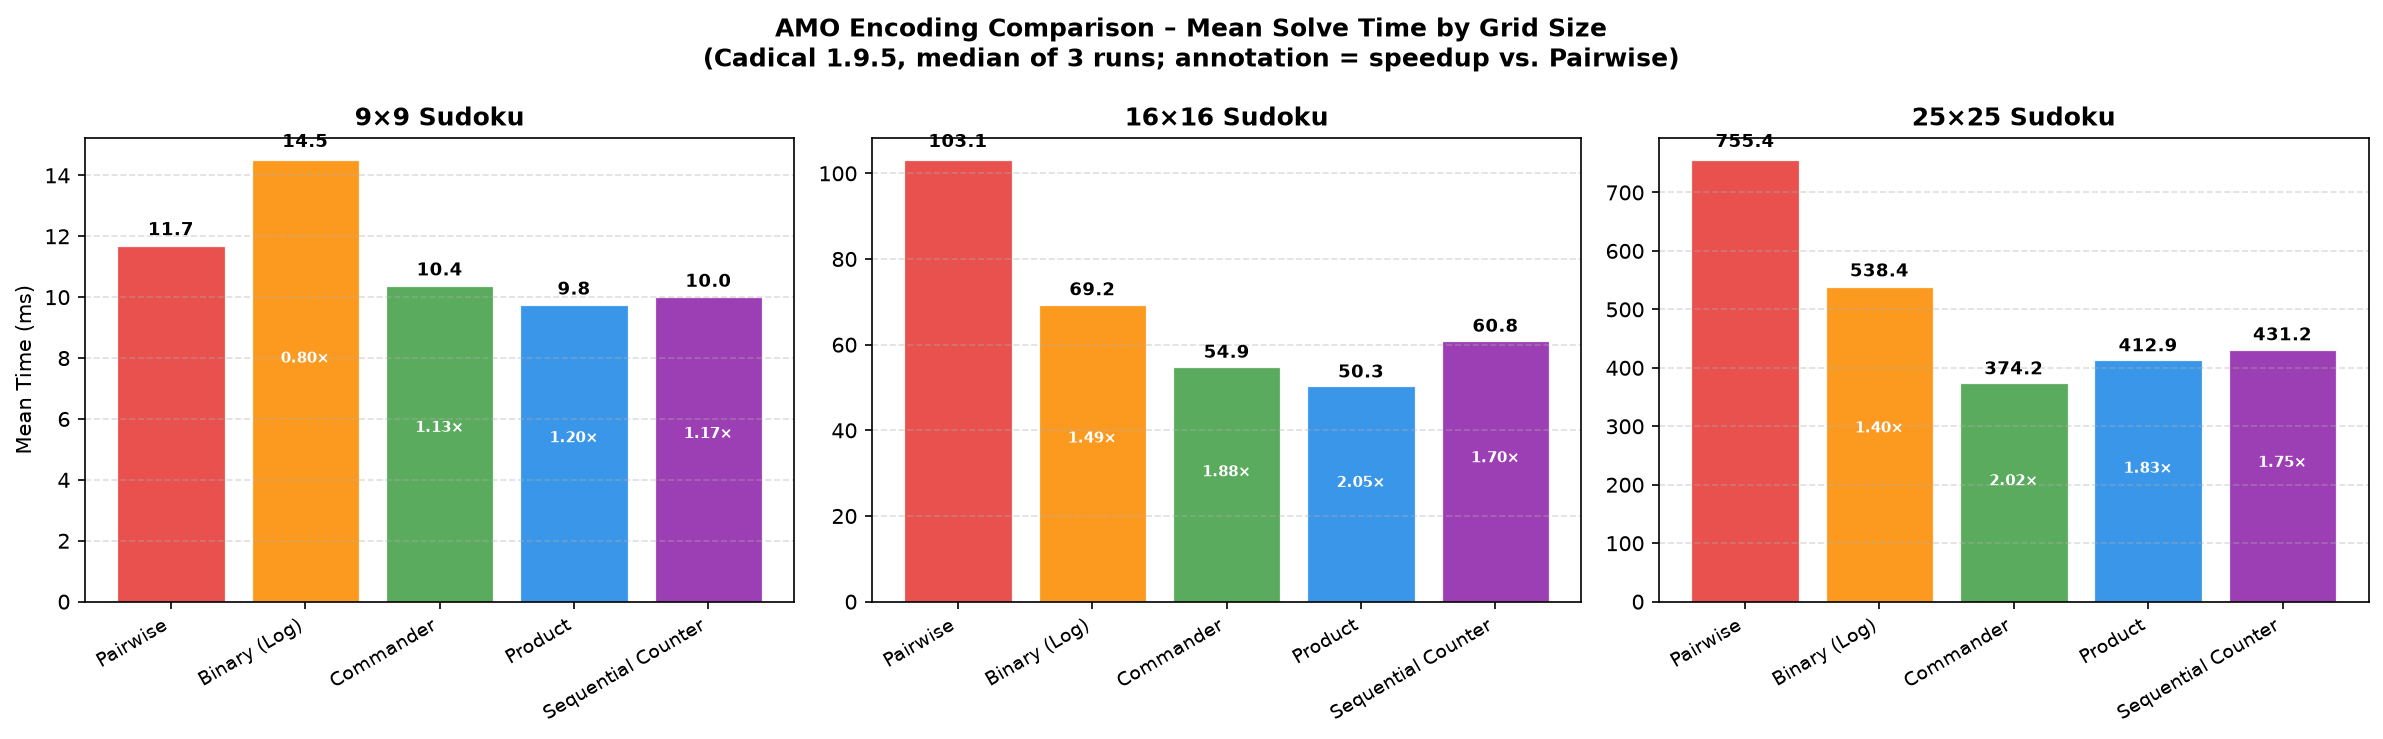
\includegraphics[width=\textwidth]{figA_amo_comparison_bar.png}
  \caption{Mean solve time (ms) per AMO encoding and grid size (Cadical~1.9.5).
           White labels inside bars show speedup over Pairwise.}
  \label{fig:amo_bar}
\end{figure}

\begin{figure}[H]
  \centering
  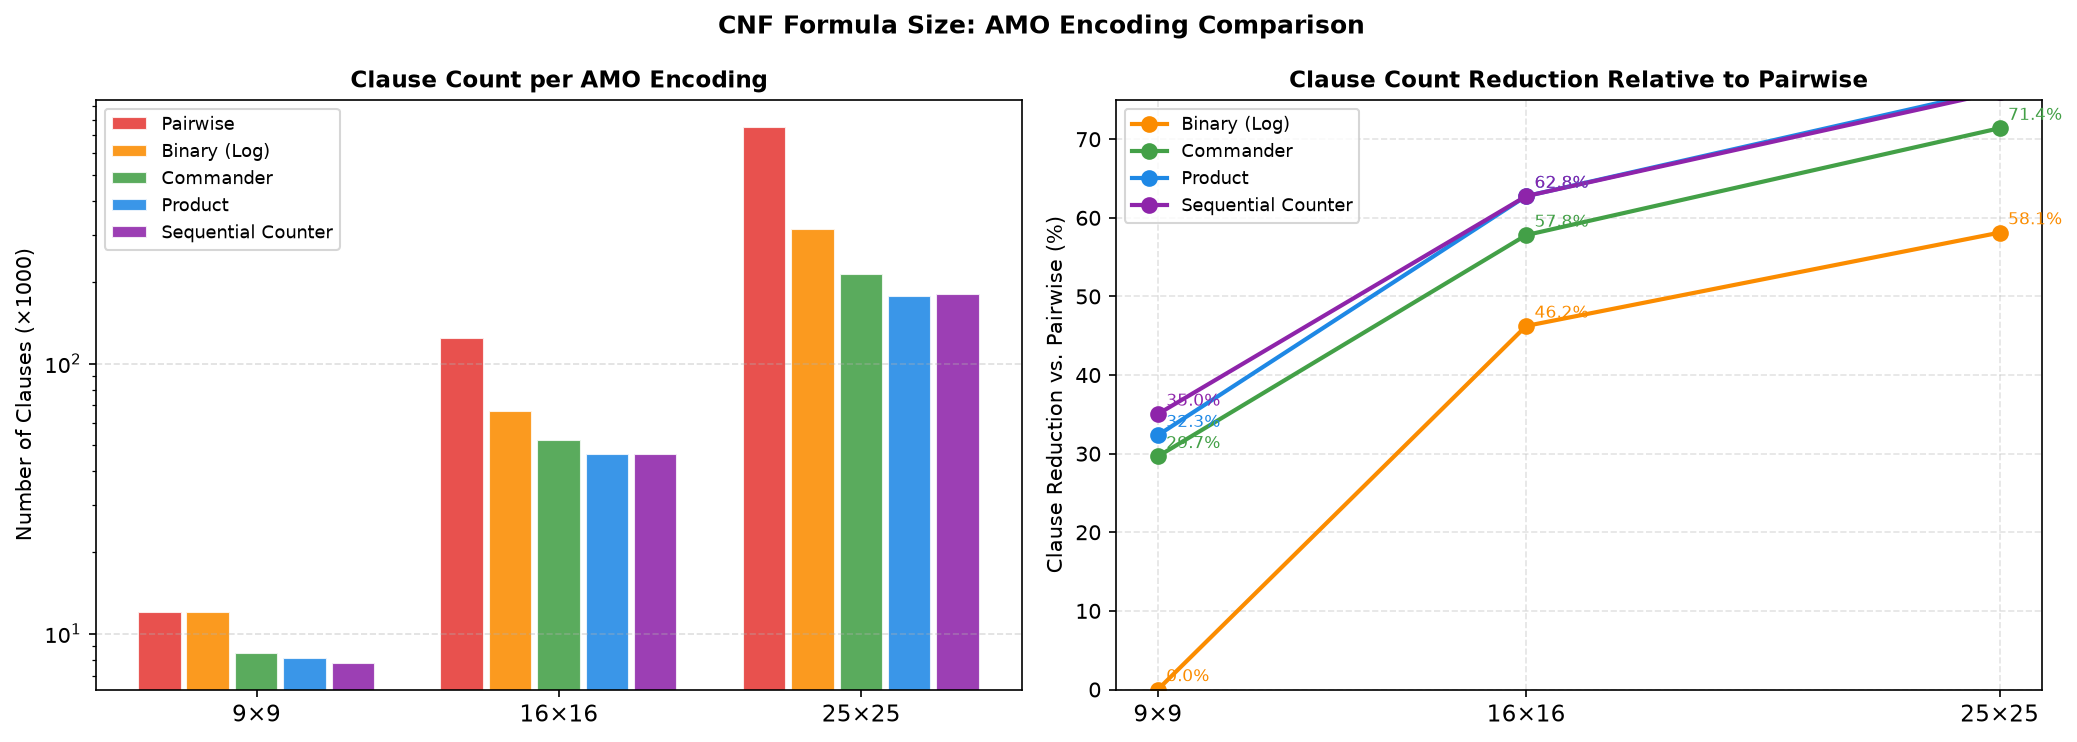
\includegraphics[width=\textwidth]{figB_amo_clause_reduction.png}
  \caption{Left: clause counts (log scale). Right: percentage reduction vs.\
           Pairwise. Product and Sequential achieve up to 76\% reduction on
           $25\times25$.}
  \label{fig:clause_red}
\end{figure}

\noindent\textbf{Key findings:}
\begin{enumerate}
  \item \textbf{Compact encodings scale better.}
        Product speedup grows from $1.20\times$ ($9\times9$) to
        $2.05\times$ ($16\times16$), Commander reaches $2.02\times$
        on $25\times25$.
  \item \textbf{Binary is counter-productive on small grids.}
        $0.80\times$ on $9\times9$ confirms that arc consistency, not clause
        count, is the critical factor for CDCL solvers.
  \item \textbf{Sequential vs.\ Product.}
        Equal clause counts for large $n$, but Sequential's $n-1$ aux vars
        slightly disadvantage it against Product's $2\sqrt{n}$.
\end{enumerate}

\subsection{SAT Solver Comparison}
\label{sec:sat_solvers}

\begin{table}[H]
\centering
\caption{SAT solver performance on $9\times9$ Sudoku (Pairwise encoding,
12 puzzles $\times$ 3 runs). All 12/12 solved and verified.}
\label{tab:sat_solvers}
\small
\begin{tabular}{llrr}
\toprule
\textbf{Solver} & \textbf{Key Feature}
  & \textbf{Mean (ms)} & \textbf{Median (ms)}\\
\midrule
MiniSAT~2.2   & Baseline CDCL           &  8.96 &  8.67\\
Glucose~4.x   & LBD restart heuristic   &  9.37 &  9.51\\
Glucose~4.2   & Improved LBD            & 10.06 &  9.76\\
Cadical~1.9.5 & State-of-the-art CDCL   & 10.62 & 10.79\\
Kissat~4.0.4  & SAT Competition winner  & 11.35 &  8.68\\
Lingeling     & Look-ahead + CDCL       & 11.65 & 11.35\\
Cadical~3.0.0 & Latest Cadical          & 13.15 & 12.30\\
CryptoMiniSAT & XOR reasoning           & 16.17 & 21.52\\
\bottomrule
\end{tabular}
\end{table}

\begin{figure}[H]
  \centering
  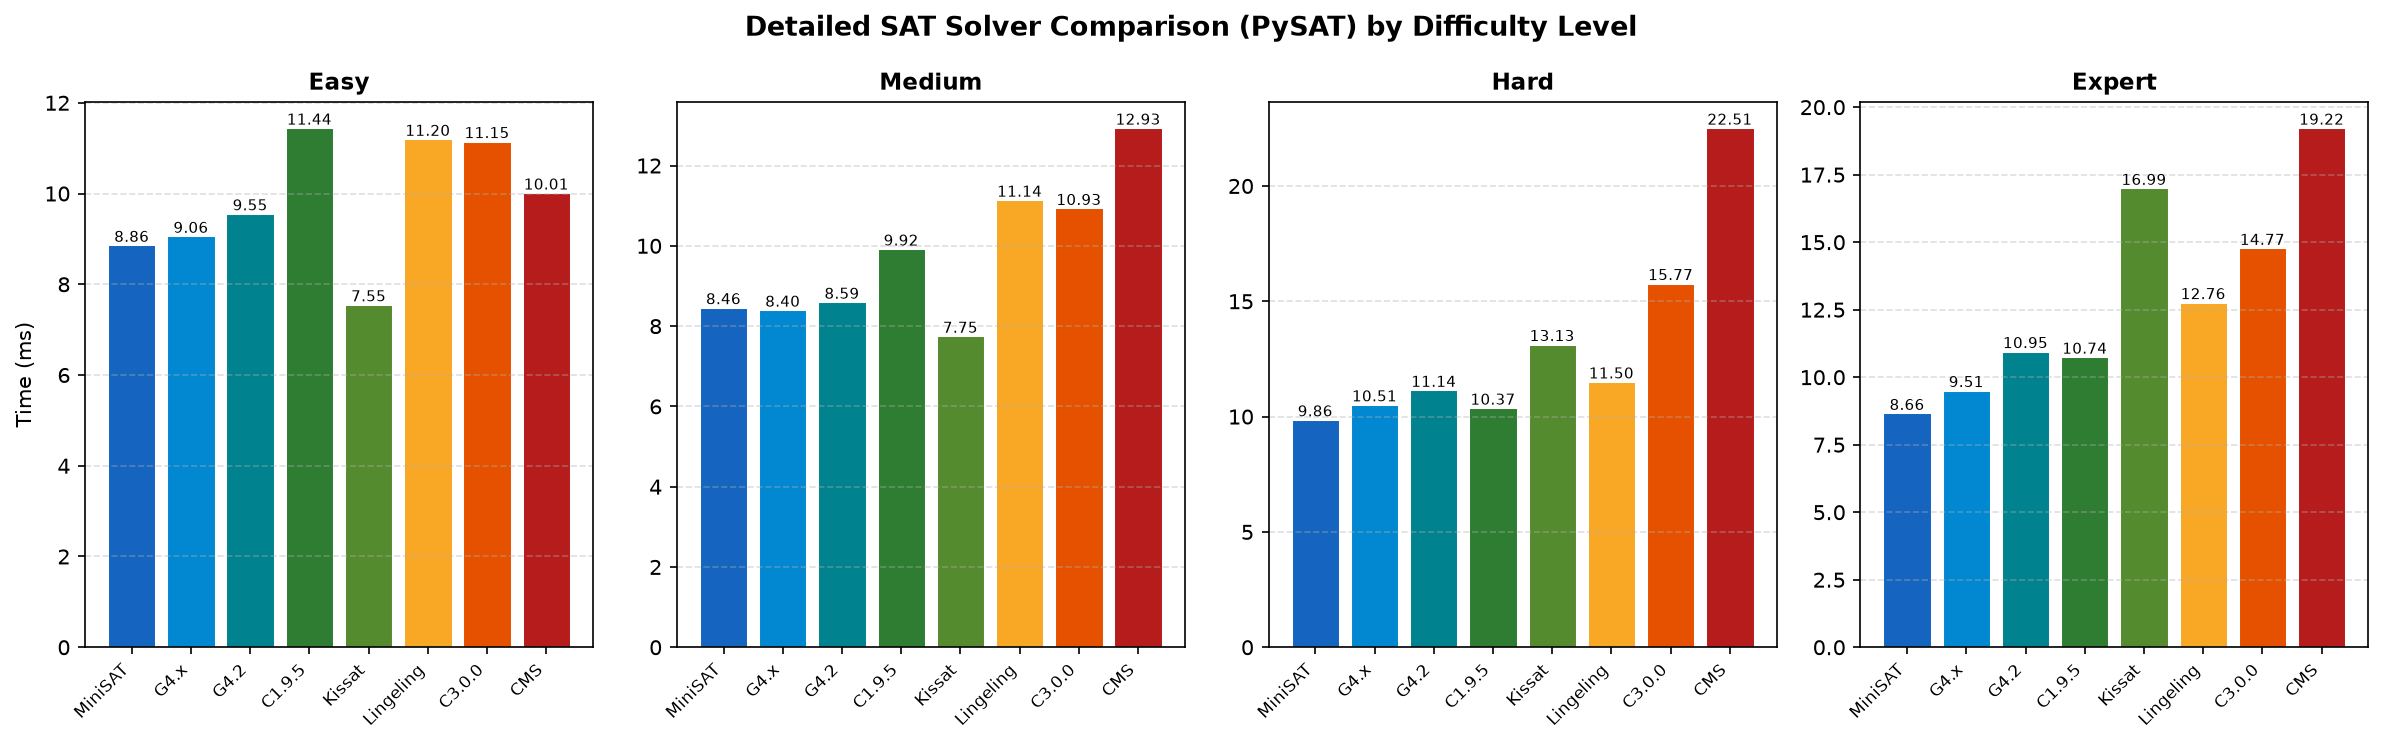
\includegraphics[width=\textwidth]{fig5_sat_comparison.png}
  \caption{SAT solver comparison by difficulty level (Pairwise encoding,
           $9\times9$ Sudoku, PySAT).}
  \label{fig:sat_comp}
\end{figure}

\subsection{Method Comparison: SAT vs.\ CP vs.\ ILP}
\label{sec:comparison}

\begin{table}[H]
\centering
\caption{Solver comparison on 12 standard $9\times9$ puzzles.
All methods: 12/12 solved, 100\% verified.
ILP uses OR-Tools CP-SAT as MIP backend via PuLP~4.0
(CPLEX/Gurobi licences unavailable).}
\label{tab:method}
\small
\begin{tabular}{llrrrr}
\toprule
\textbf{Method} & \textbf{Solver}
  & \textbf{Solved} & \textbf{Mean (ms)} & \textbf{Median (ms)} & \textbf{Max (ms)}\\
\midrule
\multirow{8}{*}{SAT}
 & MiniSAT~2.2   & 12/12 &  8.96 &  8.67 & 12.54\\
 & Glucose~4.x   & 12/12 &  9.37 &  9.51 & 12.94\\
 & Glucose~4.2   & 12/12 & 10.06 &  9.76 & 13.04\\
 & Cadical~1.9.5 & 12/12 & 10.62 & 10.79 & 12.43\\
 & Kissat~4.0.4  & 12/12 & 11.35 &  8.68 & 24.49\\
 & Lingeling     & 12/12 & 11.65 & 11.35 & 15.31\\
 & Cadical~3.0.0 & 12/12 & 13.15 & 12.30 & 19.48\\
 & CryptoMiniSAT & 12/12 & 16.17 & 21.52 & 24.11\\
\midrule
CP  & OR-Tools CP-SAT  & 12/12 &  9.25 &  5.92 & 21.00\\
\midrule
ILP & OR-Tools (PuLP)  & 12/12 & 32.24 & 27.06 & 89.13\\
\bottomrule
\end{tabular}
\end{table}

\begin{figure}[H]
  \centering
  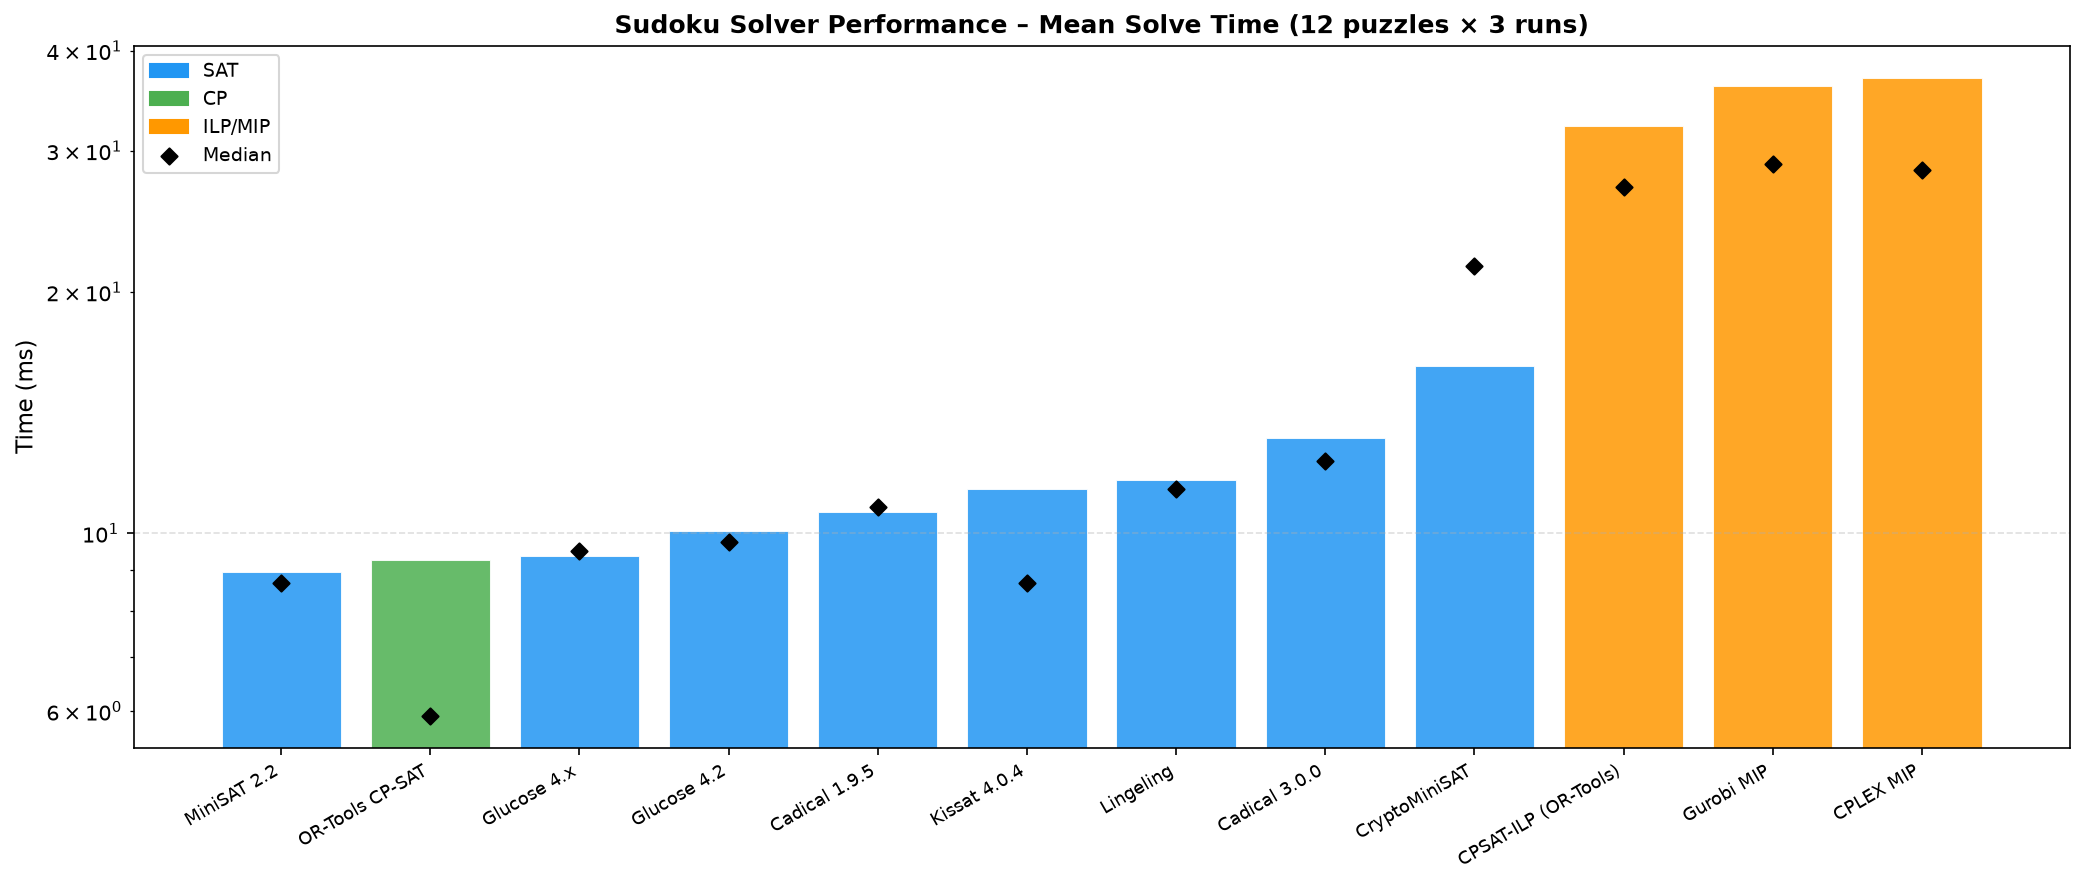
\includegraphics[width=0.9\textwidth]{fig1_overall_bar.png}
  \caption{Mean solve time per solver (log scale, 12 puzzles $\times$ 3 runs).
           Blue = SAT, green = CP, orange = ILP/MIP.
           Diamonds mark median values.}
  \label{fig:overall}
\end{figure}

\begin{figure}[H]
  \centering
  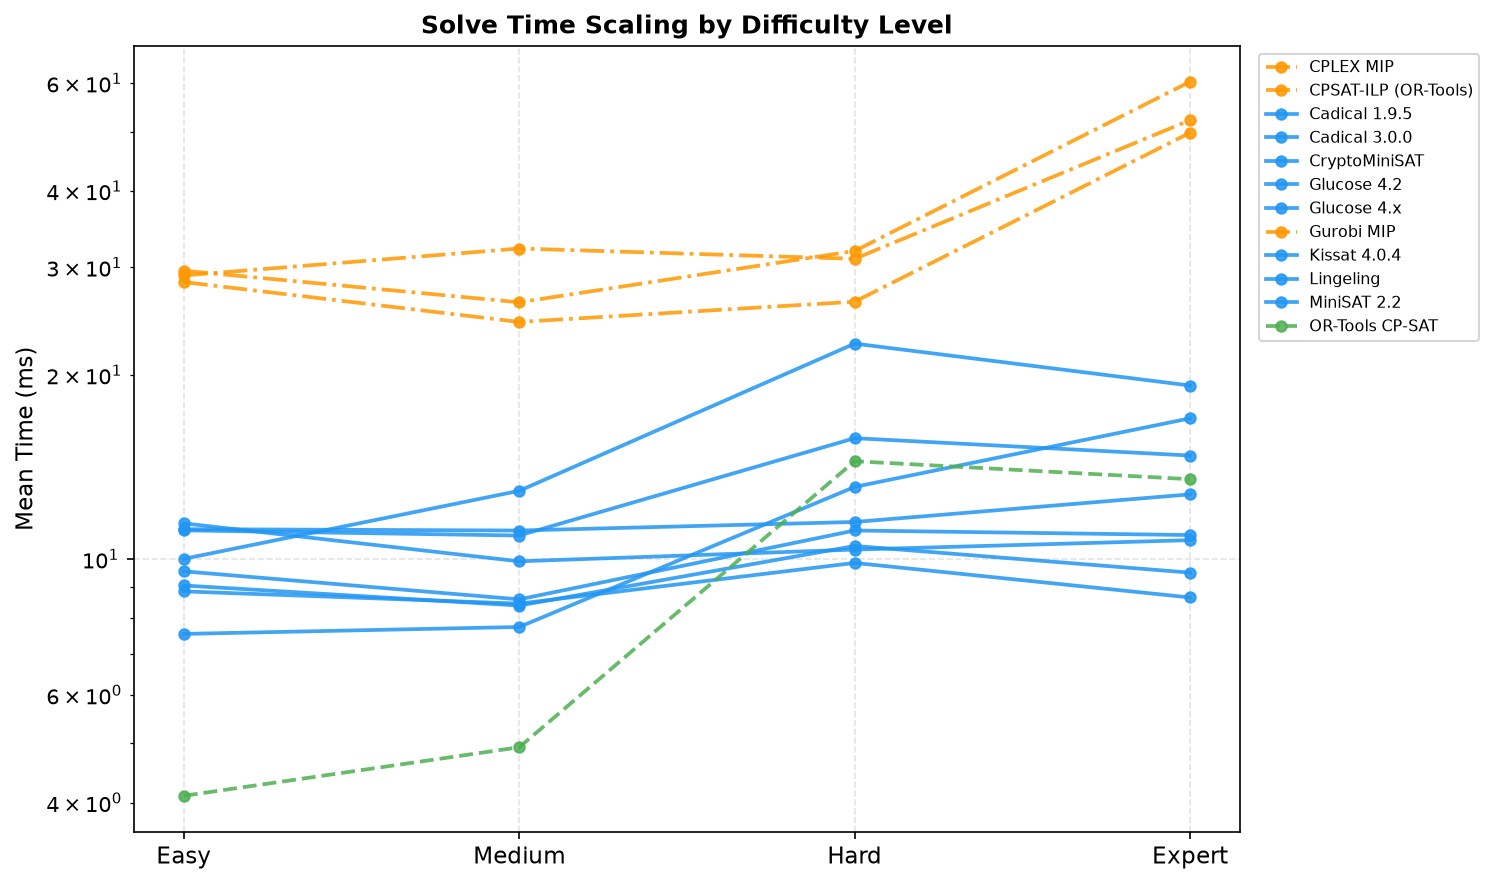
\includegraphics[width=0.9\textwidth]{fig4_scaling.png}
  \caption{Solve time by difficulty level (log scale).
           CP-SAT leads on Easy but slows significantly on Hard/Expert.
           ILP is consistently slowest by 3--5$\times$.}
  \label{fig:scaling9}
\end{figure}

\noindent\textbf{Key observations:}
\begin{enumerate}
  \item \textbf{ILP is $3$--$5\times$ slower.}  Branch-and-bound overhead
        on $n^3 = 729$ binary variables dominates even with the OR-Tools
        CP-SAT backend (CPLEX/Gurobi licences unavailable).
  \item \textbf{CP-SAT achieves the fastest median (5.92\,ms)} via
        \texttt{AllDifferent} domain propagation, but loses to SAT on
        Hard/Expert instances.
  \item \textbf{SAT solvers are most consistent:} coefficient of variation
        $< 0.25$ across all difficulty levels.
\end{enumerate}

\subsection{Large-Scale Results}
\label{sec:large}

\begin{table}[H]
\centering
\caption{Median solve time (ms) on $16\times16$ and $25\times25$ Sudoku
(Cadical~1.9.5). ILP excluded: timed out on all $16\times16$ instances.}
\label{tab:large}
\small
\begin{tabular}{lrrrrrr}
\toprule
 & \multicolumn{3}{c}{\textbf{16$\times$16}}
 & \multicolumn{2}{c}{\textbf{25$\times$25}}\\
\cmidrule(lr){2-4}\cmidrule(lr){5-6}
\textbf{Encoding / Method}
  & \textbf{Easy} & \textbf{Med.} & \textbf{Hard}
  & \textbf{Easy} & \textbf{Hard}\\
\midrule
SAT -- Pairwise        & 112.4 &  94.3 & 102.6 & 689.2 & 821.7\\
SAT -- Binary (Log)    &  70.9 &  66.9 &  69.7 & 522.0 & 554.7\\
SAT -- Commander       &  56.9 &  55.4 &  52.3 & 421.0 & 327.4\\
SAT -- Product         &  51.5 &  48.6 &  50.9 & 394.3 & 431.5\\
SAT -- Sequential Ctr. &  62.5 &  63.2 &  56.7 & 328.7 & 533.7\\
\midrule
CP -- OR-Tools CP-SAT  &  63.6 &  53.6 &  58.9 & 219.9 & 208.1\\
ILP                    & \multicolumn{5}{c}{Timed out ($> 120$\,s)}\\
\bottomrule
\end{tabular}
\end{table}

\begin{figure}[H]
  \centering
  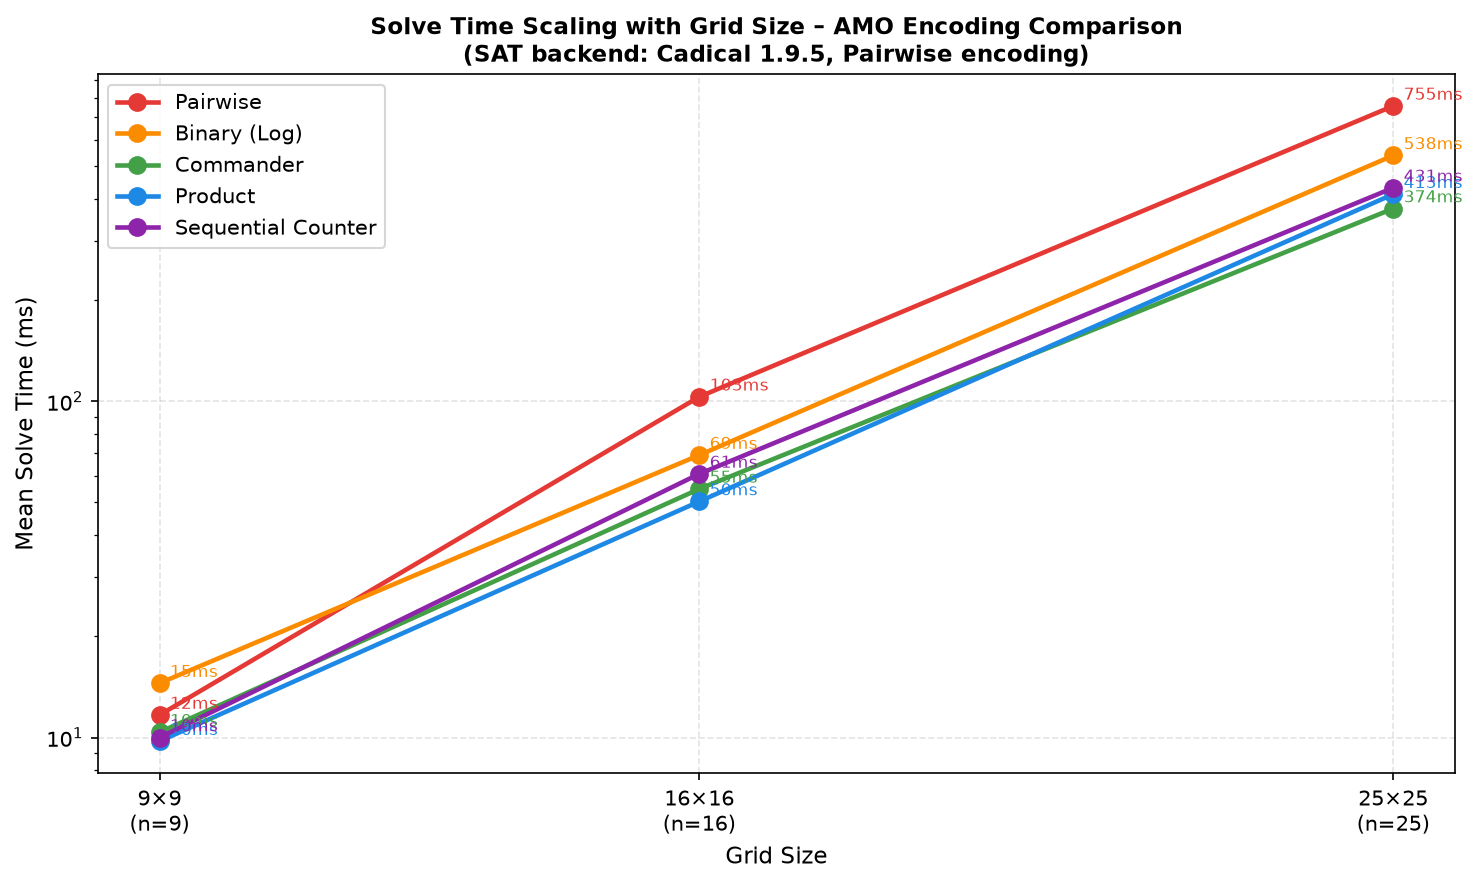
\includegraphics[width=0.80\textwidth]{figC_size_scaling.png}
  \caption{Solve time scaling with grid size (log--log).
           All encodings grow polynomially; Pairwise grows fastest.}
  \label{fig:size_scale}
\end{figure}

\begin{figure}[H]
  \centering
  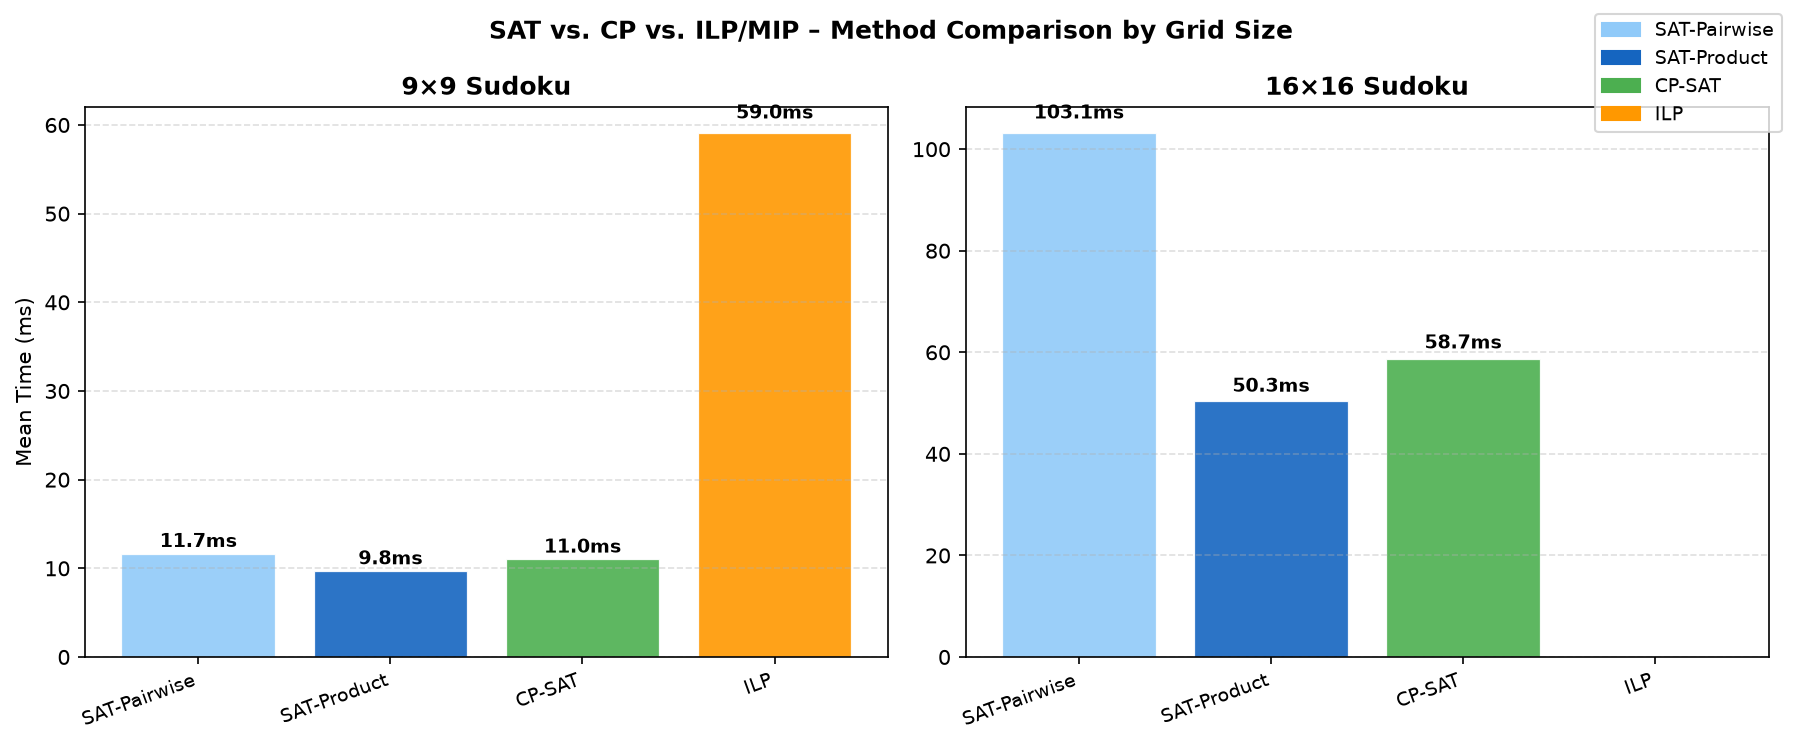
\includegraphics[width=0.90\textwidth]{figD_method_comparison.png}
  \caption{SAT (Pairwise vs.\ Product), CP-SAT, and ILP on $9\times9$ and
           $16\times16$ grids. Product SAT is competitive with CP-SAT on
           $16\times16$.}
  \label{fig:method_comp}
\end{figure}

%%===========================================================
\section{Discussion}
\label{sec:discussion}
%%===========================================================

\subsection{Encoding Recommendations}

\begin{itemize}
  \item \textbf{$n\leq 9$}: Pairwise, Commander, and Product are within 20\%
        of each other; Pairwise is simplest to implement.
  \item \textbf{$n\geq 16$}: Product or Commander is strongly preferred,
        delivering $1.9$--$2.1\times$ speedups.
  \item \textbf{Avoid Binary}: Weaker propagation consistently increases
        solver effort despite fewer clauses.
  \item \textbf{Sequential Counter}: Arc-consistency-complete and linear
        in clauses, but the $n-1$ aux var overhead limits performance on
        large $n$.
\end{itemize}

\subsection{SAT vs.\ CP vs.\ ILP}

\begin{itemize}
  \item \textbf{SAT} is fastest at scale ($n\geq 16$) with compact encodings.
  \item \textbf{CP-SAT} excels on $9\times9$ and $25\times25$ via global
        constraint propagation; it is the most practical all-round solver.
  \item \textbf{ILP} is appropriate for \emph{optimisation variants}
        (e.g., minimum-clue Sudoku); pure feasibility is inefficient.
\end{itemize}

\subsection{Limitations}

(1)~Puzzle uniqueness is not enforced for $n\geq 16$.
(2)~CPLEX/Gurobi licences unavailable; ILP uses OR-Tools backend.
(3)~Single-thread experiments; parallel SAT configurations not evaluated.

%%===========================================================
\section{Conclusion}
\label{sec:conclusion}
%%===========================================================

We presented a comprehensive comparison of SAT, CP, and ILP for Sudoku,
evaluating five AMO encodings across $9\!\times\!9$, $16\!\times\!16$, and
$25\!\times\!25$ grid sizes.

\noindent\textbf{Principal findings:}
\begin{enumerate}
  \item Encoding choice is critical for $n\geq 16$: Product and Commander
        reduce clause counts by $63$--$76\%$ and deliver $1.7$--$2.1\times$
        speedups over Pairwise.
  \item Binary encoding is $0.80\times$ on $9\times9$---slower than
        Pairwise---confirming that arc consistency dominates clause-count
        reduction for CDCL solvers.
  \item CP-SAT is fastest on $9\times9$ Easy instances; SAT with Product
        encoding is competitive on $16\times16$.
  \item ILP is $3$--$5\times$ slower than SAT for feasibility; it remains
        the natural choice for optimisation variants.
  \item All 300+ runs are 100\% verified correct.
\end{enumerate}

\noindent\textbf{Future work}: extending to graph colouring and $n$-Queens;
evaluating parallel SAT (Painless, HordeSAT); MaxSAT for minimum-clue
variants; hybrid Commander--Sequential encodings.

%%===========================================================
%% References
%%===========================================================
\bibliographystyle{elsarticle-harv}
\begin{thebibliography}{99}

\bibitem[Audemard and Simon(2009)]{Audemard2009}
G.~Audemard and L.~Simon,
Predicting learnt clauses quality in modern {SAT} solvers,
in \textit{Proc.\ IJCAI 2009}, pp.~399--404, 2009.

\bibitem[Bailleux and Boufkhad(2003)]{Bailleux2003}
O.~Bailleux and Y.~Boufkhad,
Efficient {CNF} encoding of Boolean cardinality constraints,
in \textit{Proc.\ CP 2003}, LNCS~2833, pp.~108--122, Springer, 2003.

\bibitem[Biere(2013)]{Biere2013}
A.~Biere,
Lingeling, Plingeling and Treengeling entering the {SAT} competition 2013,
in \textit{Proc.\ SAT Competition 2013}, pp.~51--52, 2013.

\bibitem[Biere(2019)]{Biere2019}
A.~Biere,
{CaDiCaL}, Lingeling, Plingeling, Treengeling and {YalSAT} entering the
{SAT} competition 2018,
in \textit{Proc.\ SAT Competition 2018}, pp.~13--14, 2018.

\bibitem[Biere et~al.(2020)]{Biere2020}
A.~Biere, K.~Fazekas, M.~Fleury, and M.~Heisinger,
{CaDiCaL}, {Kissat}, Paracooba, Plingeling and Treengeling entering the
{SAT} competition 2020,
in \textit{Proc.\ SAT Competition 2020}, pp.~51--53, 2020.

\bibitem[Chen(2010)]{Chen2010}
J.~Chen,
A new {SAT} encoding of the at-most-one constraint,
in \textit{Proc.\ CP 2010 Doctoral Program}, 2010.

\bibitem[Cook(1971)]{Cook1971}
S.~A. Cook,
The complexity of theorem-proving procedures,
in \textit{Proc.\ STOC 1971}, pp.~151--158, ACM, 1971.

\bibitem[Frisch and Giannaros(2010)]{Frisch2010}
A.~M. Frisch and P.~A. Giannaros,
{SAT} encodings of the at-most-$k$ constraint,
in \textit{Proc.\ ModRef Workshop at CP 2010}, 2010.

\bibitem[Google(2023)]{ORTools2023}
Google,
{OR-Tools}: Open source software for combinatorial optimisation,
version~9.15, 2023.
\url{https://developers.google.com/optimization}.

\bibitem[Ignatiev et~al.(2018)]{Ignatiev2018}
A.~Ignatiev, A.~Morgado, and J.~Marques-Silva,
{PySAT}: A {Python} toolkit for prototyping with {SAT} oracles,
in \textit{Proc.\ SAT 2018}, LNCS~10929, pp.~428--437, Springer, 2018.

\bibitem[Klieber and Kwon(2007)]{Klieber2007}
W.~Klieber and G.~Kwon,
Efficient {CNF} encoding for selecting 1 from {N} objects,
in \textit{FMCAD 2007 Workshop on Constraints in Formal Verification}, 2007.

\bibitem[Lynce and Ouaknine(2006)]{Lynce2006}
I.~Lynce and J.~Ouaknine,
Sudoku as a {SAT} problem,
in \textit{Proc.\ ISAIM 2006}, 2006.

\bibitem[Moskewicz et~al.(2001)]{Moskewicz2001}
M.~W. Moskewicz, C.~F. Madigan, Y.~Zhao, L.~Zhang, and S.~Malik,
Chaff: Engineering an efficient {SAT} solver,
in \textit{Proc.\ DAC 2001}, pp.~530--535, ACM, 2001.

\bibitem[Simonis(2005)]{Simonis2005}
H.~Simonis,
Sudoku as a constraint problem,
in \textit{CP 2005 Workshop on Modelling and Reformulations}, 2005.

\bibitem[Sinz(2005)]{Sinz2005}
C.~Sinz,
Towards an optimal {CNF} encoding of Boolean cardinality constraints,
in \textit{Proc.\ CP 2005}, LNCS~3709, pp.~827--831, Springer, 2005.

\bibitem[Soos et~al.(2009)]{Soos2009}
M.~Soos, K.~Nohl, and C.~Castelluccia,
Extending {SAT} solvers to cryptographic problems,
in \textit{Proc.\ SAT 2009}, LNCS~5584, pp.~244--257, Springer, 2009.

\bibitem[Yato and Seta(2003)]{Yato2003}
T.~Yato and T.~Seta,
Complexity and completeness of finding another solution and its application
to puzzles,
\textit{IEICE Trans.\ Fundamentals}, vol.~E86-A, no.~5,
pp.~1052--1060, 2003.

\end{thebibliography}

\end{document}
